\documentclass[10pt,twocolumn,letterpaper]{article}

\usepackage{statcourse}
\usepackage{times}
\usepackage{epsfig}
\usepackage{graphicx}
\usepackage{amsmath}
\usepackage{amssymb}

% Include other packages here, before hyperref.

% If you comment hyperref and then uncomment it, you should delete
% egpaper.aux before re-running latex.  (Or just hit 'q' on the first latex
% run, let it finish, and you should be clear).
\usepackage[breaklinks=true,bookmarks=false]{hyperref}


\statcoursefinalcopy


\setcounter{page}{1}
\begin{document}


%%%%%%%%%%%%%%%%%%%%%%%%%%%%%%%%%%%%%%%%%%%%%%%%%%%%%%%%%%%%%%%
% DO NOT EDIT ANYTHING ABOVE THIS LINE
% EXCEPT IF YOU LIKE TO USE ADDITIONAL PACKAGES
%%%%%%%%%%%%%%%%%%%%%%%%%%%%%%%%%%%%%%%%%%%%%%%%%%%%%%%%%%%%%%%



%%%%%%%%% TITLE
\title{Comparative Analysis of Machine Learning Models: \\Alexnet, VGG, Resnet, YOLO}

\author{Pham Duc An\\
{\tt\small 10422002}
\and
Tran Hai Duong\\
{\tt\small 10422021}
\and
Vo Thi Hong Ha\\
{\tt\small 10421015}
\and
Nguyen Hoang Anh Khoa\\
{\tt\small 10422037}
\and
Truong Hao Nhien\\
{\tt\small 10422062}
\and
Nguyen Song Thien Phuc\\
{\tt\small 10422067}\\
\\
\{\tt @student.vgu.edu.vn\}
\and
Bui Duc Xuan\\
{\tt\small 10422085}
}

\maketitle
%\thispagestyle{empty}



% MAIN ARTICLE GOES BELOW
%%%%%%%%%%%%%%%%%%%%%%%%%%%%%%%%%%%%%%%%%%%%%%%%%%%%%%%%%%%%%%%


%%%%%%%%% ABSTRACT
\begin{abstract}
   In this project, we conducted a comprehensive comparative analysis of prominent machine learning models, namely Alexnet, VGG, Resnet, and YOLO, with a focus on their efficacy in image recognition. Leveraging a curated dataset representative of diverse real-world scenarios with CIFAR-10, our study delved into the nuances of each model's architecture, training process, and computational requirements. Through rigorous evaluation using metrics such as accuracy, precision, and recall, our results reveal nuanced performance distinctions. Notably, Resnet demonstrated superior accuracy, VGG excelled in feature extraction, YOLO showcased real-time efficiency, and Alexnet exhibited a stable performance. These findings provide valuable insights for practitioners and researchers seeking to optimize model selection for specific applications, shedding light on the trade-offs between accuracy, computational cost, and real-time processing capabilities. Project's detailed code are provided at {\url{https://github.com/nhientruong04/LIA-introCS-proj}}.
\end{abstract}

%%%%%%%%% BODY TEXT
\subsection{AlexNet}
In 2012, the ImageNet Large Scale Visual Recognition Challenge (ILSVRC) \footnote{\url{https://image-net.org/challengehttps://image-net.org/challenges/LSVRC/index.phps/LSVRC/index.php}} dataset was introduced, which required a model capable of processing a large dataset like ImageNet. The introduction of Alexnet by Alex Krizhevsky, Ilya Sutskever, and Geoffrey E. Hinton marked a significant milestone in the field of computer vision. Alexnet showed the feasibility of deep learning so well that it got a top-five error of fifteen point three percent on data that has a thousand categories in the ILSVRC 2012\cite{krizhevsky_2012_imagenet}. Its original paper is the theoretical basis for the report below.
\subsubsection{Overall architecture}


\begin{flushleft}
    \begin{figure}[h!]
    \begin{center}
        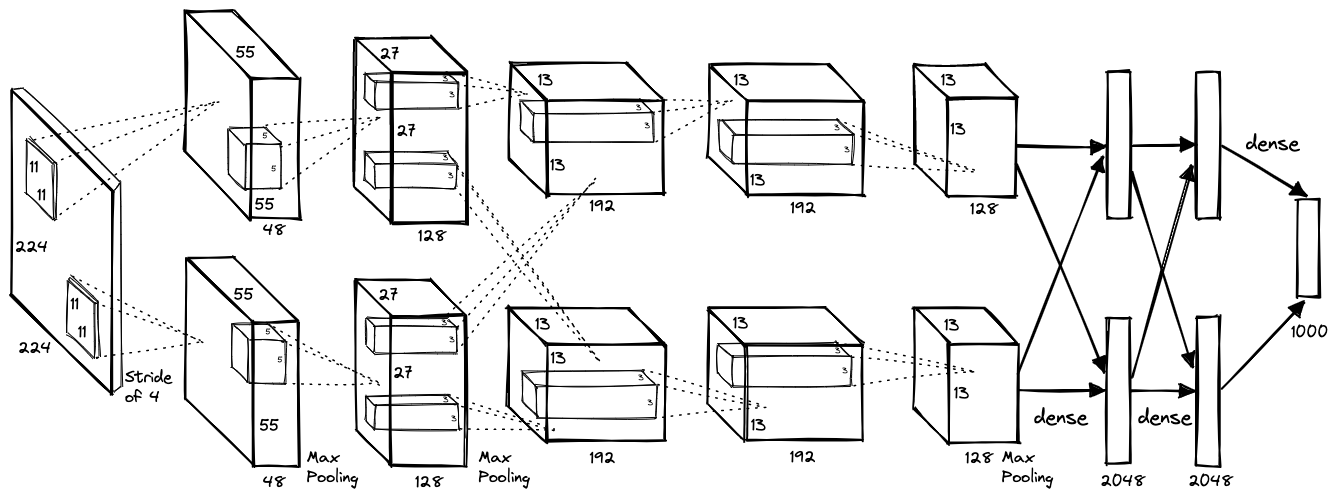
\includegraphics[scale=0.15]{imagenet-6}
        \caption{An illustration of the architecture of}{AlexNet\footnote{The input size is mentioned at most of the places as 224*224*3 but due to some special reason which happens it works out to be 227*227*3.}}{, clearly demonstrating the division of responsibility between the two GPUs.}
        \label{fig:imagenet-6}
    \end{center}
    \end{figure}
\end{flushleft}
Alexnet is a deep convolutional neural network that has 8 layers with learnable parameters. It consists of 5 convolutional layers and 3 fully connected layers. The first two Convolutional layers are followed by the pooling layers which are used to perform max pooling. The third, fourth, and fifth convolutional layers are connected directly. The Alexnet architecture takes images of size 227*227 as input and has three layers based on the RGB. After going through each layer, the number of filters becomes the kernels in the output feature map. The structure involves an increase in the number of filters as we go deeper into the architecture. The filter size is also reduced, which means the initial filter was larger. The first layers can recognize simple features, like edges, shapes, and textures. As the network gets deeper, it produces more abstract representations, eventually identifying concepts from mammals to dogs and even Siberian huskies \cite{shipra_2021_alexnet}. In the end, fully connected layers are used to produce the 1000-label classification needed for ImageNet. The output of the last fully-connected layer is fed to a 1000-way softmax which produces a distribution over the 1000 class labels\cite{krizhevsky_2012_imagenet}.



\subsubsection{ReLu activation function}

\begin{flushleft}
    
\begin{figure}[h!]
    \begin{center}
        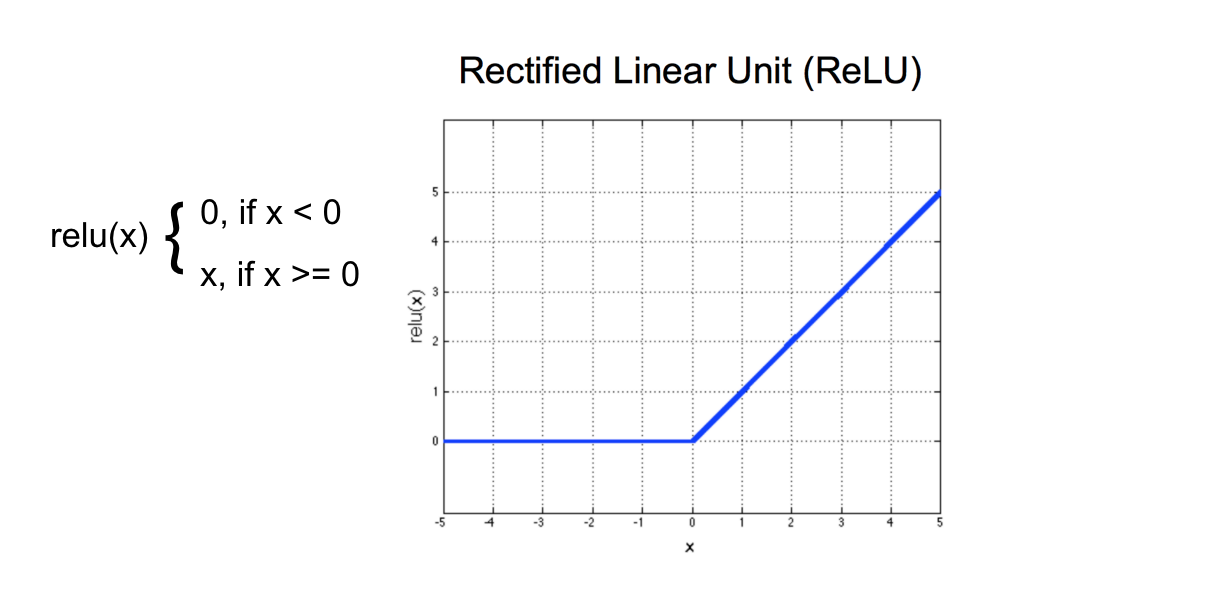
\includegraphics[scale=0.35]{relu_ex}
        \caption{ReLU activation function in the}{positive interval is always 1.}
        \label{fig:relu_ex}
    \end{center}
\end{figure}
\end{flushleft}
The AlexNet architecture introduced the use of ReLU (Rectified Linear Unit) Nonlinearity, which is a more efficient activation function than the previously used Tanh or sigmoid functions. It can be represented as: f(x) = max(0, x), where x is the input value. The paper shows that using ReLUs, AlexNet could achieve a 25\% training error rate six times faster than an equivalent network using tanh. This was tested on the CIFAR-10 dataset\cite{krizhevsky_2012_imagenet}. The function is applied after all the convolution and fully connected layers.

\subsubsection{ Multi(2)-GPU learning}
Multi-GPU learning is a method that allows for the parallelization of the training process across multiple GPUs. The authors utilized two GPUs to increase the network size, as the GPU at that time had a memory limit of 3GB. The network is split into two such as Figure \ref {fig:imagenet-6}, which communicated in specific layers to ensure they were not training two separate models. Therefore, the two-GPU net takes slightly less time to train than the one-GPU net.

\subsubsection{Dropout}
Dropout is a regularization technique that helps to prevent overfitting by randomly setting some neurons to zero during the training process. In AlexNet, dropout is applied to the first two fully-connected layers with a dropout rate of 0,5. This means that half of the neurons in these layers are ignored during each iteration of training. Dropout helps to improve the generalization performance of AlexNet on large-scale image recognition tasks.

\begin{flushleft}
    
\begin{figure}[h!]
    \begin{center}
        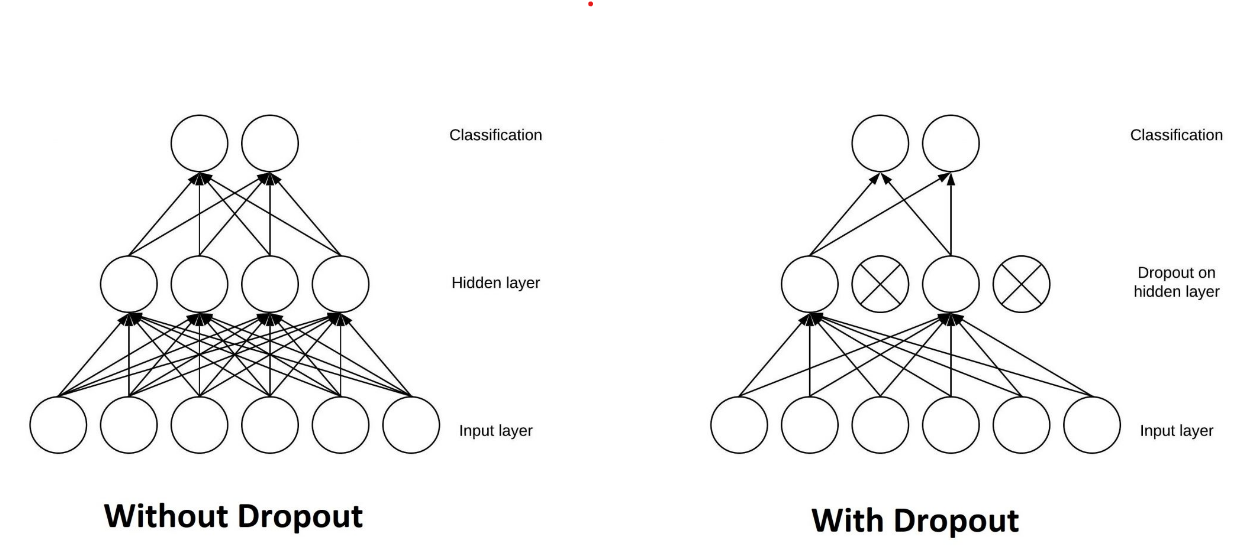
\includegraphics[scale=0.3]{dropout}
        \caption{Dropout Neural Net Model\cite{baeldung_2020_how}.}
        \label{fig:dropout}
    \end{center}
\end{figure}
\end{flushleft}


{\small
\bibliographystyle{ieee}
\bibliography{bibliography.bib}
}

\end{document}